\documentclass{article}
\usepackage[utf8]{inputenc}
\usepackage{graphicx}
\usepackage{enumerate}
\usepackage{amsmath}
\usepackage{parskip}
\usepackage{siunitx}

\usepackage{geometry}
 \geometry{
 a4paper,
 total={170mm,257mm},
 left=20mm,
 top=20mm
 }

\title{TP: Base station power consumption optimisation}
\author{Markus Säynevirta}
\date{June 2022}

\begin{document}

\thispagestyle{plain}

\large
\textbf{RIO207 - Ingénierie radio}

\large
TP: Base station power consumption optimisation\\
\textit{Markus Säynevirta}
\vspace{0.5cm}

\section{Cumulative distribution function versus SINR}
The cumulative distribution function in figure \ref{fig:q1_sinr_vs_cdf} describes the relationship probabilities of getting a certain SINR value in a given scenario.

\begin{figure}[!htb]
    \centering
    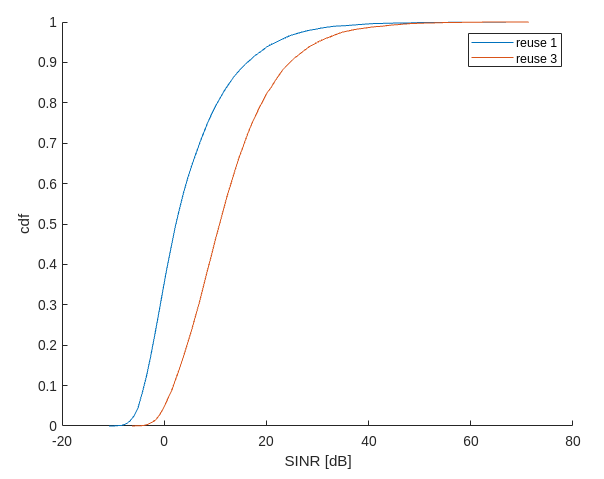
\includegraphics[width=12cm]{images/q1_sinr_vs_cdf.png}
    \caption{Cumulative distribution function in relation to SINR in the two reuse scenarios.}
    \label{fig:q1_sinr_vs_cdf}
\end{figure}

As we can see in the figure, reuse 3 graph is shifted towards higher SINR values (i.e. to the right) in relation to the graph of scenario reuse 1. This means that we're going to generally attain better SINR figures by implementing reuse 3.

\section{Computing system parameters with queueing theory}
\label{processor_sharing}

We will start by computing a set of necessary system parameters by utilising the single server waiting line model.

Average data rate \(R_u\) can be computed by solving the Shannon theorem for the weighted arithmetic mean of SINR figures given as parameter. As the probability values are normalized to 1, the weighted mean can be calculated from the simplified formula \(\bar{\gamma} = \sum S \cdot P\). Cell capacity can be calculated from the formula
\begin{gather*}
    C = W_c \log_2(1 + \bar{\gamma})
\end{gather*}

where \(W_c\) is the bandwidth of the cell.

\newpage
The other three return values can be computed from the given parameters and the previously computed average cell data rate by using formulas
\begin{gather*}
    \lambda_{max} = \frac{R_u}{B} \\
    \rho = \frac{\lambda \cdot B}{R_u} \\
    K = \frac{\lambda \cdot B}{R_u - \lambda \cdot B}
\end{gather*}

\(\lambda_{max}\), \(\rho\) and \(K\) correspond to the maximum allowable arrival rate, load and average number of active users. \(\lambda\) and \(B\) are the arrival rate in hertz and file size required to serve an individual user in bits.

Below excerpt from a Matlab printout demonstrates the price paid for the higher SINR in the case of reuse 3.

\texttt{reuse: 1 \\
Ru: 39212559.2767 maxlambda = 19.6063 rho = 0.11272 K = 0.12704 \\
reuse: 3 \\
Ru: 27888573.9238 maxlambda = 13.9443 rho = 0.15849 K = 0.18834}

As can be seen, average cell data rate is about \SI{11.3}{Mbits\per \second} slower in the latter case, the maximum allowable arrival rate is about 5.7 users per second lower while cell loading and average time required to serve an individual user are about 4.6 percentage points and 48 percent higher.

\section{Computing the outage probability}

Outage probability can be can be computed by dividing the amount of samples where the SINR figure is higher than the given threshold, dividing it by the total number of samples and subtracting the result from one. Outage probabilities for the situations with reuse 1 and reuse 3 were 0.95\ \% and 0\ \% respectively. As can be seen, the higher SINR of the reuse 3 situation shows a clear improvement in the outage probability.

The average SINR can be computed for the UEs with figures above the threshold value by taking the mean of the numerator of the array of the outage probability calculation.

\section{Computing power consumption}
The missing power figures can be computed from the following equations
\begin{gather*}
    P_{cd} = K_u R_u (P_{cod} + P_{dec}) \\
    P_{bh} = K_u R_u P_{bt} \\
    P_{circuit} = P_{fix} + P_{tc} + P_{ce} + P_{cd} + P_{bh} + P_{lp} \\
    P_{fab,bts} = \\
    P_{tot} =\rho \frac{P_{tx}}{\eta} + P_{m} + P_{c}
\end{gather*}

Here \(P_{cd}\), \(P_{bh}\), \(P_{circuit}\), \(P_{fab,bts}\) and \(P_{tot}\) are the missing power figures and refer to coding and decoding power, backhaul power, circuit power, depreciated fabrication power and the total power consumption respectively. \(P_{cod}\) and \(P_{dec}\) refer to the intrinsic coding and decoding powers in \si{\watt\per(\giga b\per\second)}. Parameters \(K_u\) and \(R_u\) are the average cell data rate and the average time required to serve a user calculated in section \ref{processor_sharing}. Other power figures have been outlined in more detail in the exercise instructions, lecture slides and the referenced paper discussing manufacturing power.

We can now calculate the power figures for the different reuse cases.

\texttt{reuse: 1 \\
Ptot: 408.3421 Ptx: 5.7668 Pfab: 380.5175 Pcircuit: 22.0578 \\
reuse: 3 \\
Ptot: 410.6767 Ptx: 8.1083 Pfab: 380.5175 Pcircuit: 22.0509}

As can be seen, total power consumption figures are very similar between the two cases with only a very minor difference arising from the different transmission power consumptions due. These differences are caused by the different figures for \(\rho\) used in the calculation of transmission power.

\section{Power consumption versus transmission power}
Power consumption of the two reuse cases over a wider envelope \texttt{in.powvect = [15 16:5:46 50]}. Figure \ref{fig:q5_Ptx_vs_Ptot} presents power consumption in Watts in relation to transmit power in dBm for the two reuse scenarios.

\begin{figure}[!htb]
    \centering
    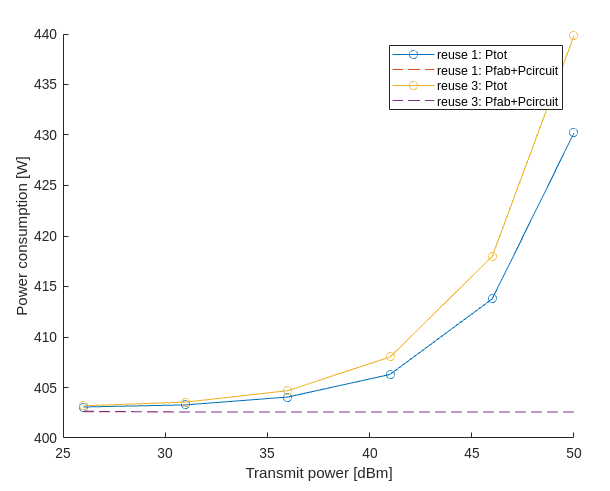
\includegraphics[width=12cm]{images/q5_Ptx_vs_Ptot.png}
    \caption{Power consumption versus transmit power in the two reuse scenarios.}
    \label{fig:q5_Ptx_vs_Ptot}
\end{figure}

As we can see from the figure, manufacturing and circuit power consumptions are identical between the two reuse options and remain constant over the transmission power envelope. Accelerating trend of the total power consumption in both scenarios is to be expected considering the logarithmic nature of the transmission power figures.

\newpage
\section{Outage probability versus transmission power}

Figure \ref{fig:q6_Ptx_vs_outage} visualises outage probabilities in relation to transmit power for the two frequency reuse scenarios.

\begin{figure}[!htb]
    \centering
    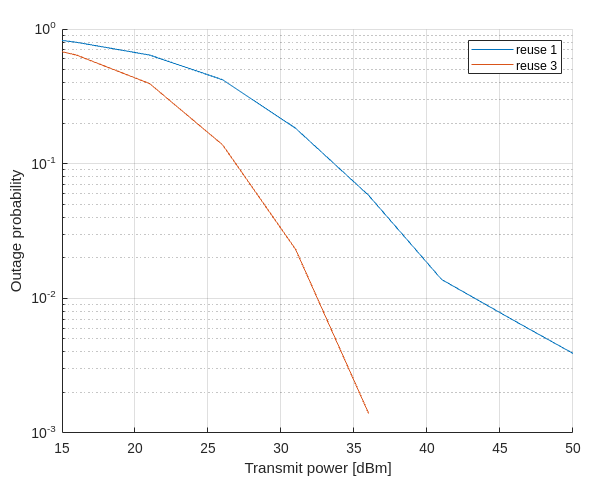
\includegraphics[width=12cm]{images/q6_Ptx_vs_outage.png}
    \caption{Outage probabilities versus transmit power in the two reuse scenarios.}
    \label{fig:q6_Ptx_vs_outage}
\end{figure}

When considering the target probability of \(< 1\ \%\), the figure shows a clear advantage for reuse 3. Examining the graphs closer gives transmit power values of 43 and \SI{32}{\decibel m} for reuse 1 and 3 respectively when considering the target outage probability. In this case, reuse 3 is clearly the better option due to its significantly lower power consumption.

\section{Throughput with modified QoS constraints}

The simulation was modified by lowering the outage probability threshold from -7 to \SI{-13}{\decibel}. The figure \ref{fig:q7_Ptx_vs_throughput} visualises throughput in relation to the transmission power in the modified simulation scenario.

\begin{figure}[p]
    \centering
    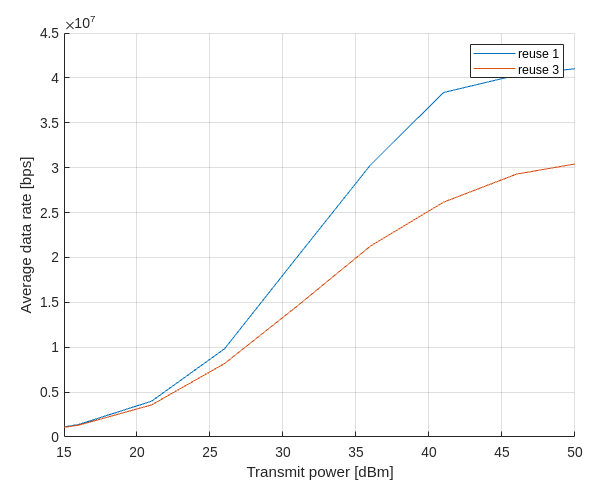
\includegraphics[width=12cm]{images/q7_Ptx_vs_throughput.png}
    \caption{Throughput versus transmit power in the modified simulation scenario.}
    \label{fig:q7_Ptx_vs_throughput}
\end{figure}

Examining the graphs, we can deduce that the required throughput can be reached at transmit powers of 33 and \SI{39}{\decibel m} for reuse 1 and 3 respectively. Consedering these numbers, reuse 1 is the better option overall as it results in a lower power consumption.

\section{Depreciation and total power consumption}
Figure \ref{fig:q8_time_vs_Ptoty} presents the total power consumption in relation to different periods of amortisation.

\begin{figure}[p]
    \centering
    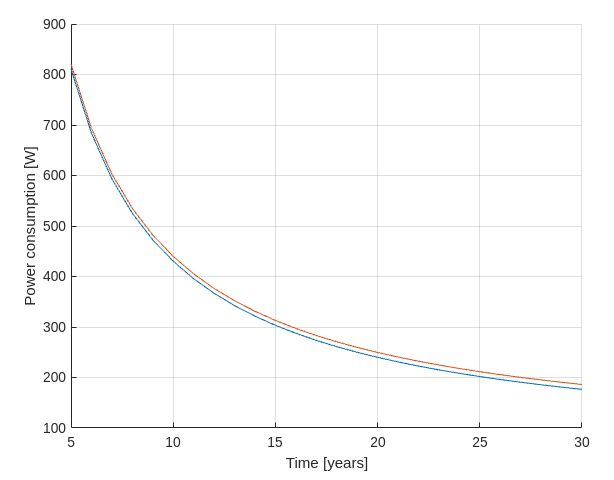
\includegraphics[width=12cm]{images/q8_time_vs_Ptoty.png}
    \caption{Total power consumption vs different periods of amortisation.}
    \label{fig:q8_time_vs_Ptoty}
\end{figure}

As can be seen, lenghtening the amortisation period has initially rather strong effect on the overall power consumption as manufacturing power consumption dominates the overall figure. On the other hand, in the long term the effect starts to diminish. Graphs of reuse 1 and reuse 3 follow each other very closely.

\newpage
\section{Energy consumption of a new versus old system}

Figure \ref{fig:q9_Ptx_vs_Ptot_new} presents the relationship of total power consumption in relation to transmission power for the new system. The same relatinship is visualised for the old system in \ref{fig:q5_Ptx_vs_Ptot}.

\begin{figure}[!htb]
    \centering
    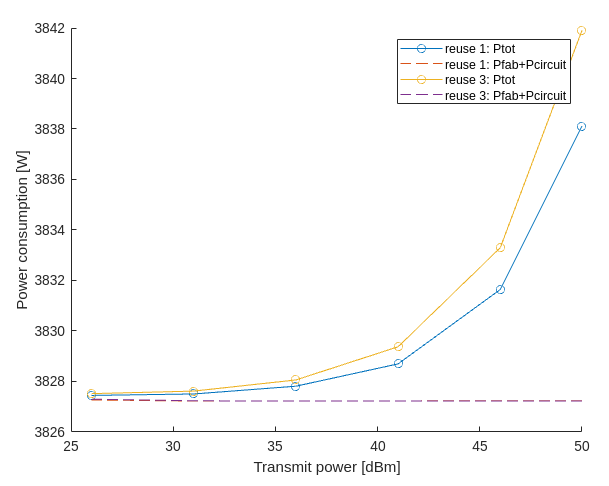
\includegraphics[width=12cm]{images/q9_Ptx_vs_Ptot_new.png}
    \caption{Power consumption versus transmit power in the two reuse scenarios for the new system.}
    \label{fig:q9_Ptx_vs_Ptot_new}
\end{figure}

As can be seen comparing the two, the baseline power consumption is much greater for the new system due to the overwhelmingly large effect of the manufacturing power. It is worth though also to compare the difference in the total power consumption between the lowest and highest transmit power. The new basestation has a difference between the top and the bottom value of around \SI{14}{W} while the difference in the old system is over two and half times greater at around \SI{37}{W}.

\end{document}
